\section{Objective}

The purpose of this lab is to introduce and learn the concept of APIs. API stands for Application Programming Interface and is defined as a set of routines, protocols, and tools for building software applications. For this particular lab, you will be using the Android SDK API.

For this lab, you will be using the \verb=MediaPlayer= and \verb=MediaRecorder= classes. These classes contain methods that utilize the Android's microphone and speakers to play and record media. Before you begin the activity, visit \textit{http://developer.android.com/reference/android/media/MediaPlayer.html} and \textit{http://developer.android.com/reference/android/media/MediaRecorder.html}. Familiarize yourself with both of these classes and their methods.

The alarm system app should be able to listen for sound and, if detected, sound an alarm. There will be three different choices for the alarm sound. The following picture shows the GUI (graphical user interface) of the app:

\begin{center}

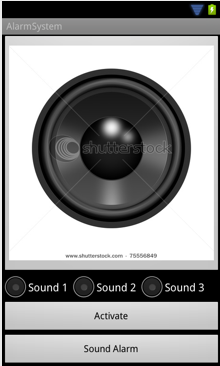
\includegraphics[scale=0.4]{screenshot.png} 

\end{center}

Both the speaker picture and the sound alarm buttons will be programmed to sound the alarm when clicked. The activate button will be programmed to begin listening for sound when clicked.
